\section{Fundamental regions}

We have seen in Remark~\ref{rem_NatureMoebius} that considering M�bius transformations as meromorphic functions $\EC \to \EC$ very naturally induces a group action of $\PGL{\C}$ on $\EC$. Clearly this group action is also given for any subgroup of $\PGL{\C}$ and in particular for the modular group: For $A = \smallmat{a}{b}{c}{d} \in \PSL{\Z}$ the group action is
\begin{equation}
\label{eqn_ModGrpAction}
Az := \moebius{a}{b}{c}{d}{z}.
\end{equation}

We are now interested in subsets of $\EC$ which contain exactly on point $z_0$ of each orbit $[z]_\sim \in \EC/\sim$:

\begin{definition}[Fundamental set]
\label{dfn_FundamentalSet}
\index{Fundamental!set}
Let $G$ be a group acting on the set $\mathcal{S}$. Denote equivalence of points in $\mathcal{S}$ under $G$ by $\sim$, as in (\ref{eqn_GroupActionEquivalence}). A subset $\mathcal{F} \subseteq \mathcal{S}$ is called a \emph{fundamental set} with respect to the group action of $G$ on $\mathcal{S}$, if $\mathcal{F}$ contains exactly one point from each orbit, \ie the map $\mathcal{F} \to \mathcal{S}/\sim$, $x \mapsto [x]_\sim$ is bijective.
\end{definition}

\begin{remark}
Fundamental sets always exist, but they are not unique in any way. If $\mathcal{F}$ is a fundamental set, then for every subset $X \subseteq \mathcal{F}$ and for every $g \in G$, also the set $(\mathcal{F} \setminus X) \cup gX$ is fundamental.
\end{remark}

If -- like in the case of $\EC$ -- the set $\mathcal{S}$ comes together with a topology defined on it, it is often advantageous to use a concept slightly different to fundamental sets:

\begin{definition}[Fundamental region]
Let $G$ be a group acting on a set $\mathcal{S}$ which is (a subset of) a topological space. A nonempty open subset $\mathcal{F} \subseteq \mathcal{S}$ is called \emph{fundamental region} with respect to the group action of $G$ on $\mathcal{S}$, if it contains no distinct points equivalent under $G$ and if the neighborhood of every boundary point of $\mathcal{F}$ contains a point of $\mathcal{S} \setminus \mathcal{F}$, which is equivalent to a point of $\mathcal{F}$.
\end{definition}

\begin{remark}
The relation of fundamental sets and fundamental regions is the following: If $\mathcal{F} \subseteq \mathcal{S}$ is a fundamental region, then its topological closure $\overline{\mathcal{F}}$ contains a fundamental set $\mathcal{F}^\ast$:
\begin{equation*}\mathcal{F} \subseteq \mathcal{F}^\ast \subseteq \overline{\mathcal{F}}.
\end{equation*}
In other words, a fundamental set $\mathcal{F}^\ast$ can always be obtained from a fundamental region $\mathcal{F}$ by adjoining certain boundary points of $\mathcal{F}$.

\index{Discontinuity}
However, a fundamental region must not always exist: Consider the group of translations $z \mapsto z + \alpha$, $\alpha \in \R$, acting on the complex plane $\C$. No matter how we arrange a fundamental set $\mathcal{F}^\ast$, take for example the imaginary axis $\Re{z} = 0$, the interior of $\mathcal{F}^\ast$ will always be empty and thus cannot contain a fundamental region. In fact, a necessary and sufficient condition for the existence of a fundamental region is that the group action is \emph{discontinuous} on $\mathcal{S}$, \ie for every $x \in \mathcal{S}$, the orbit $Gx$ must have no accumulation point in $\mathcal{S}$ -- see \Lehner{}, Chapter IV, 1B.

Note that in \Schoeneberg{}, the term ``fundamental region'' is used for any set $X$ containing a fundamental set $\mathcal{F}^\ast$ plus some or all of its (remaining) boundary points. We prefer the above definition for being more close to the commonly used meaning of ``region'', \ie a topologically connected and open set. However, we emphasize that a fundamental region does not need to be topologically connected. 
\end{remark}

The goal of this section is to identify fundamental regions and fundamental sets for the action of the modular group on $\EC$. For this purpose it is instructive to first consider homogeneous modular transformations and their natural action on $\C^2$.

% -------------------------------------------- Subsection: The action of SL2(Z)
\subsection{The action of $\SL{\Z}$ on $\C^2$}

The homogeneous modular group $\SL{\Z}$ naturally acts on the vector space $\C^2$ by matrix-vector multiplication. Written out explicitly, for $A \in \SL{\Z}$ and $x = ({}^u_v) \in \C^2$, this group action is given by
\begin{equation*}
A x = \mat{a}{b}{c}{d} \cvec{u}{v} = \cvec{a u + b v}{c u + d v}.
\end{equation*}
We equip $\C^2$ with the standard Euclidean norm and its induced topology:
\begin{equation*}
\eucnorm{\cvec{u}{v}} := \sqrt{\abs{u}^2 + \abs{v}^2}
\end{equation*}
Let us denote the orbit of $x \in \C^2$ under $\SL{\Z}$ by 
\begin{equation}
O_x := \SL{\Z} x = \setdef{Ax}{A \in \SL{\Z}} \subseteq \C^2.
\end{equation}
We now wish to find a fundamental region with respect to action of $\SL{\Z}$ on $\C^2$. For this purpose, we need to choose exactly one vector from each of the different orbits $O_x$. In order to restrict the number of candidate vectors to an easily manageable number, we could try to first look just at vectors with minimal norm in $O_x$. The problem with this idea is that in general the orbit $O_x$ might contain vectors of arbitrary small norm -- in other words $\min{\eucnorm{O_x}}$ might in general not necessarily exist. However, in many cases it does:

\begin{lemma}[Existence of $\min{\eucnorm{O_x}}$]
\label{lem_SL2FunDomMinExists}
Let $x = ({}^u_v) \in \C^2$ be a vector with $u,v$ being linear independent over $\R$. For every $r > 0$, there are only finitely many points $y \in O_x$ with $\eucnorm{y} \le r$. In particular, $m := \min{\eucnorm{O_x}}$ exists and $m > 0$.
\end{lemma}
\begin{proof}
Since the complex numbers $u$ and $v$ are linear independent over $\R$, they span a non-degenerate parallelogram $P_x := \setdef{t u + s v}{t,s \in [0,1)}$ on the complex plane. Translation of $P_x$ by integer multiples of $u$ and $v$ covers every point in $\C$ exactly once. The set
\begin{equation}
L_x := \setdef{a u + b v \in \C}{a,b \in \Z}
\end{equation}
consists precisely of the vertices of all of these translated parallelograms. For $r > 0$, denote by $D_r$ a disk of raduis $r$ in $\C$ and by $B_r$ a ball of radius $r$ in $\C^2$ (both centered about the origin):
\begin{eqnarray}
D_r &:=& \setdefsz{\big}{z \in \C}{\abs{z} \le r},\\
B_r &:=& \setdefsz{\big}{y \in \C^2}{\eucnorm{y} \le r}.
\end{eqnarray}
Obviously $L_x \cap D_r$ is finite for every $r > 0$. Now let $r > 0$ be sufficiently large such that the set $O_x \cap B_r$ is not empty (e.g.\ $r = \eucnorm{x}$) and observe
\begin{equation*}
O_x \cap B_r \subseteq (L_x \cap D_r)^2.
\end{equation*}
We see that also the set $O_x \cap B_r$ is finite and $m = \min{\eucnorm{O_x}} = \min{\eucnorm{O_x \cap B_r}}$ therefore exists. Since $u$ and $v$ are linear independent over $\R$ (and in particular over $\Z$), $0 \notin L_x$ and consequently $0 \notin O_x$, which is why $m > 0$.
\end{proof}

We now turn to the question how we can effectively determine an element of $O_x$ with minimal norm. The task is the following: Given a vector $x = ({}^u_v) \in \C^2$ with $u,v$ linear independent over $\R$, find a matrix $B \in \SL{\Z}$ such that $\eucnorm{Bx}$ is minimal. 

In Corollary~\ref{cor_SLZandPSLZGen} we have seen that $\SL{\Z}$ is generated by the matrices $T = \smallmat{0}{-1}{1}{\phantom{-}0}$ and $U = \smallmat{1}{1}{0}{1}$. The idea is now to successively multiply $x$ with appropriate powers of $T$ and $U$ to obtain vectors of smaller and smaller norm. We do this by first finding an integer $k_0 \in \Z$, such that $\eucnorm{U^{-k_0}x}$ is minimal. Then we multiply with $T$ and repeat the process for finding $k_1 \in \Z$ minimizing $\eucnorm{U^{k_1} T U^{k_0} x}$ and so on. The procedure ends when $k_n = 0$ for some $n>0$. Note that the integers $k_j$ can be determined easily:
\begin{lemma}
\label{lem_SL2FunDomMin}
Let $x = ({}^u_v)\in \C^2$ with $v \ne 0$. The statements
\begin{enumerate}[\qquad(i)]
\item \label{itm_xMinA}
$k \in \Z$ minimizes $\eucnorm{U^{-k}x} = \eucnorm{\cvec{u - k v}{v}}$,
\item \label{itm_xMinB} $k \in \Z$ minimizes $\abs{u - k v}$,
\item \label{itm_xMinC} $k \in \Z$ minimizes $\abs{\frac{u}{v} - k}$,
\item \label{itm_xMinD} $\abs{\Re{\frac{u}{v}} - k} \le \reci{2}$,
\item \label{itm_xMinE} $k = \nint{\Re{\frac{u}{v}}}$,
\end{enumerate}
satisfy the relations $(\ref{itm_xMinA}) \Leftrightarrow (\ref{itm_xMinB}) \Leftrightarrow (\ref{itm_xMinC}) \Leftrightarrow (\ref{itm_xMinD})$ and $(\ref{itm_xMinE}) \Rightarrow (\ref{itm_xMinD})$.
\end{lemma}
\begin{proof}
Trivial.
\end{proof}
Let us now suppose that the described procedure comes to an end, \ie $k_n = 0$ for some $n > 0$. Set $B  := TU^{k_{n-1}} \cdots TU^{k_0}$ and $y :=  Bx$. It follows from $k_n = 0$ and from the choice of $k_{n-1}$ that we have 
\begin{equation}
\label{eqn_SL2FunDomLokMin}
\eucnorm{y} \le \eucnorm{U^k y} \text{\quad and \quad} \eucnorm{y} \le \eucnorm{U^k \inv{T} y} \text{\quad for all } k \in \Z.
\end{equation}
Using Lemma~\ref{lem_SL2FunDomMin} -- (\ref{itm_xMinA}) $\Leftrightarrow$ (\ref{itm_xMinD}) -- we see that (\ref{eqn_SL2FunDomLokMin}) is equivalent to
\begin{equation*}
\abs{\Re{\frac{y_1}{y_2}}} \le \reci{2} \text{\quad and \quad} \abs{\Re{\frac{y_2}{y_1}}} \le \reci{2},
\end{equation*}
which can easily be rewritten to
\begin{equation}
\label{eqn_SL2MinRegionCond}
\abs{y_1 \conj{y_2} + \conj{y_1} y_2} \le \min\{\abs{y_1}^2, \abs{y_2}^2\}.
\end{equation}
The question arises, if $y$ is just a ``local minimum'' in the sense (\ref{eqn_SL2FunDomLokMin}) or if (\ref{eqn_SL2MinRegionCond}) already implies the global minimality of $y$, \ie $\eucnorm{y} = \min \eucnorm{O_x}$. The following theorem will give us insight on this.

\begin{theorem}
\label{thm_SL2FunDomGlobMin}
Let $A \in \SL{\Z}$ be an arbitrary homogeneous modular transformation and let the \emph{grading} $n(A)$ be defined as in (\ref{eqn_grading}). Let $x = ({}^u_v) \in \C^2$ with $uv \ne 0$. Then the following statements hold:
\begin{enumerate}[(i)]
\item \label{itm_SL2FunDomGlobMinA}
If $\abs{u\conj{v} + \conj{u}v} \le \min\{\abs{u}^2,\abs{v}^2\}$, then $\eucnorm{x} \le \eucnorm{Ax}$.
\item \label{itm_SL2FunDomGlobMinB}
If $\abs{u\conj{v} + \conj{u}v} \le \min\{\abs{u}^2,\abs{v}^2\}$ and $n(A) > 3$, then $\eucnorm{x} < \eucnorm{Ax}$.
\item \label{itm_SL2FunDomGlobMinC}
If $\abs{u\conj{v} + \conj{u}v} < \min\{\abs{u}^2,\abs{v}^2\}$ and $n(A) > 2$, 
then $\eucnorm{x} < \eucnorm{Ax}$.
\end{enumerate}
\end{theorem}
\begin{proof}
Let us denote $A = \smallmat{a}{b}{c}{d}$. We need to show $\eucnorm{x} \le \eucnorm{Ax}$, that is
\begin{eqnarray*}
\abs{u}^2 + \abs{v}^2 
&\le& \abs{au + bv}^2 + \abs{cu + dv}^2 =\\
&& (au + bv)(a\conj{u} + b\conj{v}) + (cu + dv)(c\conj{u} + d\conj{v}) =\\
&& (a^2 + c^2)\abs{u}^2 + (b^2 + d^2)\abs{v}^2 + (ab + cd)(u\conj{v} + \conj{u}v),
\end{eqnarray*}
which is equivalent to
\begin{equation*}
(a^2 + c^2 - 1)\abs{u}^2 + (b^2 + d^2 - 1)\abs{v}^2 \ge -(ab + cd)(u\conj{v} + \conj{u}v).
\end{equation*}
Now we find an upper bound of the right hand side by taking its absolute value and using $\abs{u\conj{v} + \conj{u}v} \le \min\{\abs{u}^2, \abs{v}^2\} =: m$. The same time, $m$ also helps us with a lower bound of the left hand side:
\begin{equation*}
(a^2 + b^2 + c^2 + d^2 - 2) \cdot m \ge \abs{ab + cd} \cdot m.
\end{equation*}
Since $m$ is nonzero ($uv \ne 0$), it can be canceled. Moreover, $ad - bc = 1$ implies that the terms $ad$ and $bc$ can never have opposite signs. In other words we always have $(ad)(bc) \ge 0$. Obviously also $(ab)(cd) \ge 0$, \ie also the terms $ad$ and $bc$ have non-opposite signs, which is why $\abs{ab + cd} = \abs{ab} + \abs{bd}$. For this reason we can transform the last inequality to
\begin{equation}
\label{eqn_SL2FunDomIneq}
\underbrace{(a^2 - \abs{ab} + b^2)}_{\ge(\abs{a}-\abs{b})^2 =: \ell} + 
\underbrace{(c^2 - \abs{cd} + d^2)}_{\ge(\abs{c}-\abs{d})^2 =: r} \ge 2.
\end{equation}
This obviously holds for the case $n(A) = 2$. For the case $n(A) > 2$, because of $ad - bc = 1$, we see:
\begin{enumerate}[\quad(a)]
\item 
\label{itm_SL2FunDomObsA}
$\abs{a} = \abs{b}$ implies $\abs{c} \ne \abs{d}$ (and vice versa). Therefore at least one of the lower bounds $\ell$ and $r$ is nonzero.
\item 
\label{itm_SL2FunDomObsB}
$\abs{ab} = 0$ implies $\abs{bc} \ne 0$ (and vice versa). Therefore at least one of the lower bounds $\ell$ and $r$ is in fact a \emph{strict} lower bound.
\end{enumerate}
These two observations prove (\ref{eqn_SL2FunDomIneq}) and consequently assertion (\ref{itm_SL2FunDomGlobMinA}). If additionally $n(A) > 3$, we distinguish two cases:
\begin{description}
\item[Case $0 \in \{a,b,c,d\}$:] Assume without restriction that $0 \in \{a,b\}$, (the case $0 \in \{c,d\}$ is completely symmetric). It follows $\{\abs{a},\abs{b}\} = \{0,1\}$ and $\{\abs{c},\abs{d}\} = \{1,N\}$ with $N > 1$, since $n(A) > 3$. Therefore, in addition to observation (\ref{itm_SL2FunDomObsB}), both lower bounds $\ell$ and $r$ are positive. 
\item[Case $0 \notin \{a,b,c,d\}$:] In addition to observation (\ref{itm_SL2FunDomObsA}), $\abs{ab}$ and $\abs{cd}$ are both nonzero. Therefore $\ell$ and $r$ are both strict lower bounds.
\end{description}
In both cases (\ref{eqn_SL2FunDomIneq}) is strictly fulfilled, which proves (\ref{itm_SL2FunDomGlobMinB}). We note that in the case $n(A) > 3$, (\ref{itm_SL2FunDomGlobMinC}) already follows from (\ref{itm_SL2FunDomGlobMinB}). It therefore remains to consider just the special case $n(A) = 3$ for proving the last statement. By the same calculation as above, the condition $\eucnorm{x} < \eucnorm{Ax}$ is equivalent to
\begin{equation}
\label{eqn_SL2FunDomIneqB}
(a^2 + c^2 - 1)\abs{u}^2 + (b^2 + d^2 - 1)\abs{v}^2 > -(ab + cd)(u\conj{v} + \conj{u}v).
\end{equation}
For $n(A) = 3$ we have $\{(a^2 + c^2 - 1),(b^2 + d^2 - 1)\} = \{0,1\}$, which means that the left hand side simplifies to either $\abs{u}^2$ or $\abs{v}^2$, whereas on the right hand side we have $\abs{u\conj{v} + \conj{u}v}$ as upper bound, because of $(ab + cd) = \pm 1$. Since by assumption $\abs{u\conj{v} + \conj{u}v} < \min\{\abs{u}^2,\abs{v}^2\}$, inequality (\ref{eqn_SL2FunDomIneqB}) is thus satisfied.
\end{proof}

We can now summarize the algorithm and prove its correctness. Note that we can slightly relax the requirement on the coordinates of $x = ({}^u_v)$ being linear independent over $\R$. We will see that with a minor adaption the algorithm works as well in the case when $u$ and $v$ are linear dependent over $\Q$.

\begin{theorem}
\label{thm_SL2FunDomAlg}
Let $x = ({}^u_v) \in \C^2$ with $u,v$ being either linear independent over $\R$ or linear dependent over $\Q$. A matrix $B \in \SL{\Z}$ minimizing $\eucnorm{Bx}$ can be found by performing the following steps:
\begin{enumerate}
\item Set $(r_{-1},r_0) := (u,v)$ and $j := 0$.
\item \label{itm_SL2FunDomAlgLoop}
If $r_j = 0$, then goto step \ref{itm_SL2FunDomAlgDone}.
\item Determine $q_j := \nint{\Re{\frac{r_{j-1}}{r_j}}}$.
\item If $j > 0$ and $q_j = 0$ go to step \ref{itm_SL2FunDomAlgDone}. Otherwise, set $r_{j+1} := r_{j-1} - q_j r_j$, increment $j$ by one and continue with step \ref{itm_SL2FunDomAlgLoop}.
\item \label{itm_SL2FunDomAlgDone} Set $n := j-1$ and for $i \in \{0,1,\dots,n\}$, set $e_i := (-1)^i q_i$. The desired matrix is
\begin{equation}
\label{eqn_SL2FunDomMinMat}
B = U^{-e_n} TU^{-e_{n-1}} \cdots TU^{-e_0}.
\end{equation}
Note that in the case $n < 0$ this product is empty and $B$ is the identity matrix.
\end{enumerate}
\end{theorem}
\begin{proof}
The algorithm gives rise to the following sequence of equations:
\begin{IEEEeqnarray*}{rCcCl}
u &=& r_{-1} &=& q_0 \cdot r_0 + r_1 \\
v &=&    r_0 &=& q_1 \cdot r_1 + r_2 \\
&&       r_1 &=& q_2 \cdot r_2 + r_3 \\
&&       r_2 &=& q_3 \cdot r_3 + r_4 \\
&& &\vdots& 
\end{IEEEeqnarray*}
Moreover this sequence of equations corresponds to the sequence of vectors
\begin{equation*}
\cvec{u}{v}                           \overset{TU^{-q_0}}{\longmapsto}
\cvec{\phantom{+}v\phantom{_1}}{-r_1} \overset{TU^{q_1}}{\longmapsto}
\cvec{-r_1}{-r_2}                     \overset{TU^{-q_2}}{\longmapsto}
\cvec{-r_2}{\phantom{+}r_3}           \overset{TU^{q_3}}{\longmapsto}
\cvec{r_3}{r_4}                       \mapsto \dots
\end{equation*}
With $s_j := (-1)^{\ceil{\half{j}}} r_j$, we can write these vectors as $x_j := \cvec{s_{j-1}}{s_j}$ for $j \ge 0$, in particular we have $x_0 = x$. Now, as in the theorem, let $e_j := (-1)^j q_j$ for $j \ge 0$. In this notation, we can write in general $TU^{-e_j} x_j = x_{j+1}$ for all $j \ge 0$. 

In the case when $u$ and $v$ are linear dependent over $\Q$, the vector $x$ can be written as $x = \lambda ({}^p_q)$ with $\lambda \in \C$ and $p,q \in \Z$. We observe the striking similarity between the Euclidean and the above algorithm: If we apply the Euclidean algorithm to $p$ and $q$ while rounding all quotients to the nearest integer (compare Remark~\ref{rem_EuclideanAlgorithmRounding}), we obtain a sequence of quotients $\tilde{q}_0, \tilde{q}_1, \dots, \tilde{q}_n$ and a sequence of remainders $\tilde{r}_0, \tilde{r}_1, \dots, \tilde{r}_n, \tilde{r}_{n+1}$ with $\tilde{r}_{n+1} = 0$. It is immediate to see that $q_j = \tilde{q}_j$ and $r_j = \lambda \tilde{r}_j$ for all $j \ge 0$. In particular, our algorithm terminates and we end up with the vector
\begin{equation*}
y := x_n = TU^{-e_n} TU^{-e_{n-1}} \cdots TU^{-e_0} = \lambda \cvec{\pm \gcd(p,q)}{0}
\end{equation*}
having minimal norm in $O_x$.

In the case when $u$ and $v$ are linear independent over $\R$, it follows from the choice of $q_j$ that for each pair of subsequent vectors $x_j$, $x_{j+1}$ we have $\eucnorm{x_j} \ge \eucnorm{x_{j+1}}$. Using $r_{j+1} = r_{j-1} - q_j r_j$ we see that $\eucnorm{x_j} = \eucnorm{x_{j+1}}$ is equivalent to
\begin{equation*}
\eucnorm{\cvec{\pm r_{j-1}}{\pm r_{j\phantom{-1}}}} = 
\eucnorm{\cvec{\pm r_{j\phantom{+1}}}{\pm r_{j+1}}} =
\eucnorm{\cvec{\pm r_j}{\pm (r_{j-1} - q_j r_j)}}.
\end{equation*}
Obviously this is the case if and only if $\abs{r_{j-1}} = \abs{r_{j-1}-q_j r_j}$. If we divide by $r_j$ and set $z_j := \frac{r_{j-1}}{r_j}$, we obtain
\begin{eqnarray*}
\abs{z_j} = \abs{z_j - q_j} 
&\Leftrightarrow& z_j \conj{z_j} = (z_j - q_j)(\conj{z_j} -q_j)\\
&\Leftrightarrow& q_j \left(q_j - 2\Re{z_j}\right) = 0.
\end{eqnarray*}
One obvious solution to this is $q_j = 0$. For the other factor, we substitute $\alpha := \Re{z_j}$ and use $q_j = \nint{\alpha}$ to see that the equation $\nint{\alpha} = 2 \alpha$ has the unique\footnote{Here we benefit from our definition of $\operatorname{nint}$, which rounds $\pm \reci{2}$ to zero.} solution $\alpha = 0$ which again leads to $q_j = 0$. Summing up, we therefore have for all $j \ge 0$
\begin{equation}
\label{eqn_SL2FunDomAlgNormDec}
\eucnorm{x_j} \ge \eucnorm{x_{j+1}} 
\quad \text{and} \quad
\eucnorm{x_j} = \eucnorm{x_{j+1}} \Leftrightarrow q_j = 0.
\end{equation}
According to Lemma~{\ref{lem_SL2FunDomMinExists}}, the set $O_x \cap K_{\eucnorm{x}}$ is finite and thus we cannot have $\eucnorm{x_j} > \eucnorm{x_{j+1}}$ for infinitely many indices $j$. In other words, $q_n$ must be zero for some $n \in \N$ and we have
\begin{equation*}
TU^{-e_n} \cdots TU^{-e_1} TU^{-e_0} x_0 = x_n.
\end{equation*}
Since the vector $y := x_n$ satisfies (\ref{eqn_SL2FunDomLokMin}) and consequently ({\ref{eqn_SL2MinRegionCond}}), we conclude from  Theorem~\ref{thm_SL2FunDomGlobMin} that $\eucnorm{y} = \min{\eucnorm{O_x}}$. 

In both cases (linear dependence of $u,v$ over $\Q$ or linear independence over $\R$), we trivially have $\eucnorm{y} = \eucnorm{\inv{T}y}$ and we therefore can define $B$ as in ($\ref{eqn_SL2FunDomMinMat}$).
\end{proof}

Let us now denote by $\hat{\mathcal{S}} \subseteq \C^2$ the set of all vectors whose coordinates $u$ and $v$ are linear independent over $\R$ or linear dependent over $\Q$. It is clear that $\hat{\mathcal{S}}$ is invariant under the action of $\SL{\Z}$, \ie $\SL{\Z}\hat{\mathcal{S}} = \hat{\mathcal{S}}$. We can therefore as well consider the group action of $\SL{\Z}$ on $\hat{\mathcal{S}}$. We have seen in Theorem~\ref{thm_SL2FunDomGlobMin} that within the region
\begin{equation}
\label{eqn_SL2MinRegionDef}
\hat{\mathcal{R}} := \setdefsz{\bigg}{\cvec{u}{v} \in \C^2}{\abs{u\conj{v} + \conj{u}v} < \min \{\abs{u}^2, \abs{v}^2\}} \subseteq \hat{\mathcal{S}}
\end{equation}
equivalence of points can only be established by transformations $A \in \SL{\Z}$ with $n(A) = 2$. Clearly these transformations are exactly given by $1, T, T^2$ and $T^3$. On the other hand, by Theorem~\ref{thm_SL2FunDomAlg}, every vector $x \in \hat{\mathcal{S}}$ is equivalent to a point in the topological closure of $\hat{\mathcal{R}}$. Hence we can obtain a fundamental region for the group action of $\SL{\Z}$ on $\hat{\mathcal{S}}$ by choosing for each $x \in \hat{\mathcal{R}}$ exactly one of the equivalent vectors 
\begin{equation*}
x = \cvec{u}{v},\quad 
Tx = \cvec{-v}{\phantom{+}u},\quad
T^2x = \cvec{-u}{-v},\quad
T^3x = \cvec{\phantom{+}v}{-u}.
\end{equation*}
This choice can be done quite arbitrarily -- for example we can arrange the fundamental region such that the coordinates $u$ and $v$ of each of its points lie in a certain fixed halfplane of $\C$, e.g.\ $\Re{u} > 0$ and $\Re{v} > 0$.
\begin{corollary}
\label{cor_SL2FunDom}
The set
\begin{equation}
\hat{\FunDom} := \hat{\mathcal{R}} \cap \setdefsz{\bigg}{\cvec{u}{v} \in \C^2}{\Re{u}, \Re{v} > 0},
\end{equation}
where $\hat{\mathcal{R}}$ is defined as in (\ref{eqn_SL2MinRegionDef}), is a fundamental region for the action of the homogeneous modular group $\SL{\Z}$ on the set $\hat{\mathcal{S}}$.
\end{corollary}


% ------------------------------------------- Subsection: The action of PSL2(Z)
\subsection{The action of $\PSL{\Z}$ on $\EC$}

In Theorem~\ref{thm_SL2FunDomAlg} we have seen an algorithm which naturally gives rise to a set $\hat{\mathcal{R}} \subseteq \C^2$ which can easily be restricted to a subset $\hat{\FunDom} \subseteq \hat{\mathcal{R}}$ being a fundamental region for the action of $\SL{\Z}$ on $\hat{\mathcal{S}}$. We can exploit this fact in search of a fundamental region for the action on of the (inhomogeneous) modular group $\PSL{\Z}$ on $\EC$. For this purpose we project $\C^2$ onto $\EC$ using the map $\pi : \C^2 \to \EC$,
\begin{equation}
\pi : \cvec{u}{v} \mapsto \frac{u}{v}.
\end{equation}
Let us first consider image of $\hat{\mathcal{S}}$ under $\pi$. If $({}^u_v) \in \hat{\mathcal{S}}$, then by definition $u$ and $v$ are linear independent over $\R$ or linear dependent over $\Q$. In the first case we have $\frac{u}{v} \in \C \setminus \R$ and in the second case $\frac{u}{v} \in \Q \cup \{\infty\}$. This means $\frac{u}{v}$ may be everything but irrational. Denoting the set of irrational numbers by $\Irrat := \R \setminus \Q$, we thus have
\begin{equation*}
\pi(\hat{\mathcal{S}}) = \EC \setminus \Irrat.
\end{equation*}
Projection of the set $\hat{\mathcal{R}} \subseteq \C^2$ leads to the region $\mathcal{R} \subseteq \EC$ (see also Figure~\ref{fig_PSL2MinRegion}),
\begin{equation}
\label{eqn_PSL2MinRegion}
\mathcal{R} := \pi\left(\hat{\mathcal{R}}\right) = 
\setdefsz{\Big}{\frac{u}{v} \in \EC}{\abs{u\conj{v} + \conj{u}v} < \min\{\abs{u}^2, \abs{v}^2\}}.
\end{equation}
\begin{figure}
\centering
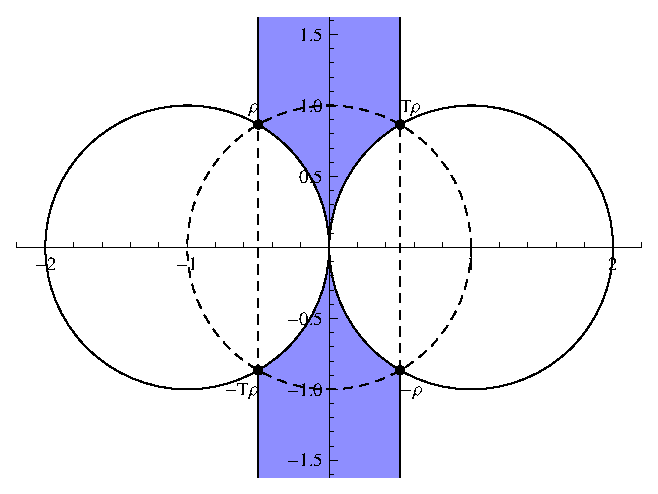
\includegraphics[width=0.8\textwidth]{figures/minimal-region}
\caption[The region $\mathcal{R} \subseteq \EC$]{The region $\mathcal{R} \subseteq \EC$ of numbers $z = u/v \in \EC$ with $\abs{u\conj{v} + \conj{u}v} < \min\{\abs{u}^2,\abs{v}^2\}$. It is obtained by taking the strip $\setdefsz{\big}{z \in \C}{\abs{\Re{z}} < \reci{2}}$  and cutting out two closed disks of unit radius centered about the real points $\pm 1$. The arising vertices are labeled. As usual, $T$ is the transformation $z \mapsto -\reci{z}$ and $\rho = \exp(2 \pi \ii / 3)$ is a third root of unity.}
\label{fig_PSL2MinRegion}
\end{figure}
It follows that $\mathcal{R}$ contains a fundamental region for the action of $\PSL{\Z}$ on $\EC \setminus \Irrat$. As in the homogeneous case, we see from Theorem~\ref{thm_SL2FunDomGlobMin} that equivalence of points within $\mathcal{R}$ can be established only by powers of the transformation $T \in \PSL{\Z}$. Since $T^2 = 1$, in order to obtain a fundamental region we now need to choose for each $z \in \mathcal{R}$ just exactly one of the equivalent points $z$ and $Tz$. This can for example be done such that $\abs{z} > 1$.

\index{Extended upper half-plane}
Note that for understanding the group action of $\PSL{\Z}$ on $\EC \setminus \Irrat$ it is sufficient to look at either the upper or lower half-plane of $\C$, since the group action on one half-plane is symmetric to the group action on the other half-plane by $A\conj{z} = \conj{Az}$. Let us therefore denote by $\mathcal{H}$ the upper half-plane and by $\EU$ the \emph{extended upper half-plane}:
\begin{eqnarray}
\label{eqn_Upperhalfplane}\mathcal{H} &:=& \setdefsz{\big}{z \in \C}{\Im{z} > 0} \\
\label{eqn_ExtUpperhalfplane}
\EU &:=& \mathcal{H} \cup \Q \cup \{\infty\}.
\end{eqnarray}
Clearly $\EU$ is invariant under $\PSL{\Z}$, \ie $\PSL{\Z} \EU = \EU$ and we can also consider $\PSL{\Z}$ acting on $\EU$.

\begin{theorem}
\label{thm_PSL2FunDom}
Let $\mathcal{H}$ and $\EU$ be defined as above. The set
\begin{equation}
\tilde{\FunDom} := \setdefsz{\bigg}{z \in \C}{\abs{\Re{z}} < \reci{2} \text{ and } \abs{z} > 1}
\end{equation}
is a fundamental region for the action of $\PSL{\Z}$ on $\EC \setminus \Irrat$. The part of $\tilde{\FunDom}$ lying in the upper half-plane $\mathcal{H}$, \ie the set
\begin{equation}
\label{eqn_PSL2FunDom}
\FunDom := \tilde{\FunDom} \cap \mathcal{H}
\end{equation}
is a fundamental region for the action of $\PSL{\Z}$ on $\EU$.
\end{theorem}
\begin{proof}
The second statement that $\FunDom = \tilde{\FunDom} \cap \mathcal{H}$ is fundamental region for $\PSL{\Z}$ acting on $\EU$ is a simple consequence of the first statement. For proving that $\tilde{\FunDom}$ is fundamental,  observe that $\tilde{\FunDom}$ is exactly the set
\begin{equation*}
\tilde{\FunDom} = \mathcal{R} \cap \setdefsz{\Big}{z \in \C}{\abs{z} > 1},
\end{equation*}
with $\mathcal{R}$ defined as in (\ref{eqn_PSL2MinRegion}) -- compare also Figure~\ref{fig_PSL2MinRegion}. Obviously $\tilde{\FunDom}$ is a nonempty open subset of $\mathcal{R}$, which is why two distinct points of $\tilde{\FunDom}$ can be equivalent only by the transformation $T$. However, since $\abs{z} > 1$ implies $\abs{Tz} = \abs{-1/z} < 1$, this is impossible. Therefore $\tilde{\FunDom}$ contains no equivalent distinct points.

It remains to show that every $z = \frac{u}{v} \in \mathcal{S}$ is equivalent to a point of the topological closure $\topcl{\tilde{\FunDom}}$ of $\tilde{\FunDom}$. For this purpose apply the algorithm of Theorem~\ref{thm_SL2FunDomAlg} to the vector $({}^u_v) \in \hat{\mathcal{S}}$ in order to obtain a transformation $B \in \PSL{\Z}$ which maps $z$ to a point of $\topcl{\mathcal{R}}$. It then follows that at least one of the points $Bz$ or $TBz$ lies in $\topcl{\tilde{\FunDom}}$.
\end{proof}

We now wish to obtain a \emph{fundamental set} for the action of $\PSL{\Z}$ on $\EU$. For this purpose we need to consider the boundary of $\FunDom$ and to investigate equivalent boundary points and their associated transformations. It turns out that we can define a fundamental set for the action of $\PSL{Z}$ on $\EU$ the following way:

\begin{theorem}[The fundamental set $\FunSet$]
\label{thm_PSL2FunSet}
Denote by $\FunDom$ the fundamental region from (\ref{eqn_PSL2FunDom}). The boundary of $\FunDom$ shall be segmented into the four ``boundary arcs'',
\begin{eqnarray*}
a &:=& \setdefsz{\bigg}{-\reci{2} + y \ii}{y \ge \frac{\sqrt{3}}{2}} \cup \{\infty\},\\
b &:=& \setdefsz{\bigg}{+\reci{2} + y \ii}{y \ge \frac{\sqrt{3}}{2}} \cup \{\infty\},\\
c &:=& \setdefsz{\Big}{\ii \cdot \epo{+\ii \phi}}{0 \le \phi \le \frac{\pi}{6}},\\
d &:=& \setdefsz{\Big}{\ii \cdot \epo{-\ii \phi}}{0 \le \phi \le \frac{\pi}{6}}.
\end{eqnarray*}
These boundary arcs are mapped onto each other by $Ua = b$ and $Tc = d$. The set
\begin{equation}
\label{eqn_PSL2FunSet}
\FunSet := \FunDom \cup a \cup c
\end{equation}
is a fundamental set for the action of $\PSL{\Z}$ on the extended upper half-plane $\EU$.
\end{theorem}
\begin{proof}
It follows from Theorem~\ref{thm_SL2FunDomGlobMin} that equivalence of boundary points of $\FunDom$ can only be established by transformations $A \in \PSL{Z}$ with $n(A) \le 3$. The full list of candidate transformations therefore comprises of 9 transformations: $T$, $U$, $TU$, $UT$, $TUT$ and the respective inverse transformations (note that $T$ is self-inverse). After looking at these transformations individually, it turns out that in fact only $T$ and $U$ (and $\inv{U}$) map boundary points to boundary points. Indeed $Ua = b$ and $Tc = d$ can readily be seen.
\end{proof}

\begin{remark}
\label{rem_PSL2FunDomGenDisks}
\begin{figure}
\label{fig_FunDomGenDisks}
\centering
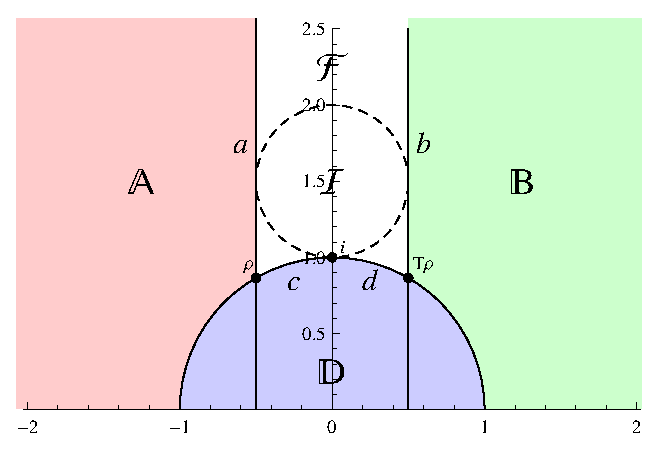
\includegraphics[width=0.8\textwidth]{figures/fundom}
\caption[The fundamental domain $\FunDom$ for the action of $\PSL{\Z}$ on $\EU$]{The fundamental domain $\FunDom$ for the action of the modular group $\PSL{\Z}$ on the extended upper half-plane $\EU$. It is bounded by ``generalized arcs'' $a$, $b$, $c$ and $d$ which correspond to the generalized disks $\mathbb{A}$, $\mathbb{B}$ and the unit disk $\mathbb{D}$. There is a unique disk $\Indisk \subseteq \FunDom$ which is tangent to $\mathbb{A}$, $\mathbb{B}$ and $\mathbb{D}$.}
\label{fig_PSL2FunDom}
\end{figure}
In Figure~\ref{fig_PSL2FunDom}, we see that the fundamental region $\FunDom$ can also be described in terms of generalized disks (see Definition~\ref{dfn_GenDisk}): With the terminology of Theorem~\ref{thm_PSL2FunSet}, the boundary arcs $a$ and $b$ are indeed ``generalized arcs'' of the closed generalized disks $\mathbb{A}$ and $\mathbb{B}$. Their defining matrices are
\begin{equation*}
\mathbb{A} : \mat{0}{1}{1}{1} \quad \text{and} \quad 
\mathbb{B} : \mat{\phantom{+}0}{-1}{-1}{\phantom{+}1}.
\end{equation*}
The boundary arcs $c$ and $d$ are part of the boundary of the closed unit disk $\mathbb{D}$, given by the matrix
\begin{equation*}
\mathbb{D} : \mat{1}{\phantom{+}0}{0}{-1}.
\end{equation*}
We see that the fundamental region $\FunDom$ can be characterized as set complement of the union of these three closed g-disks:
\begin{equation}
\label{eqn_PSL2FunDomDiskComplement}
\FunDom = \EU \setminus \left(\mathbb{A} \cup \mathbb{B} \cup \mathbb{D}\right).
\end{equation}
\end{remark}

\begin{definition}
\label{dfn_PSL2Indisk}
\index{Indisk}
Let the generalized disks $\mathbb{A}$, $\mathbb{B}$ and $\mathbb{D}$ be defined as in Remark~\ref{rem_PSL2FunDomGenDisks}. The unique (open) g-disk $\Indisk \subseteq \FunDom$, which is tangent to $\mathbb{A}$, $\mathbb{B}$ and $\mathbb{D}$ is called the \emph{indisk} $\Indisk$ of the fundamental region $\FunDom$. Its defining matrix is given by
\begin{equation}
\label{eqn_PSL2Indisk}
\Indisk : \mat{2}{-3\ii}{3\ii}{4}.
\end{equation}
\end{definition}

